%%*****************************************************************************%%
%																				%
%																				%
%								LEAVE ME HERE									%
%																				%
%																				%
%              _____ ______   ________                   _______   				%  
%             |\   _ \  _   \|\   __  \                 /  ___  \    			%
%             \ \  \\\__\ \  \ \  \|\  \  ____________ /__/|_/  /|   			%
%              \ \  \\|__| \  \ \   _  _\|\____________\__|//  / /   			%
%               \ \  \    \ \  \ \  \\  \\|____________|   /  /_/__  			%
%                \ \__\    \ \__\ \__\\ _\                |\________\			%
%                 \|__|     \|__|\|__|\|__|                \|_______|			%
%                                                      							%
%																				%
%%*****************************************************************************%%
%									Links										%
%																				%
%		x Read only : https://www.overleaf.com/read/dfghjwxtdtbv				%
%		x Edit&Read : https://www.overleaf.com/6594055mqppzz					%
%		x Github	: https://www.github.com/MR-2								%
%																				%
%%*****************************************************************************%%
%							About - This Document								%
%																				%
%		x	 RGB Venn Diagram													%
%																				%
%		Note: Use it however you want.											%
%																				%
%%*****************************************************************************%%
%									Setup										%
%																				%
\documentclass[%
    varwidth
    ,float=false % this is the new default and can be left away.
    ,preview=true
    ,class=scrartcl
    ]{standalone}
\usepackage[rgb]{xcolor}
\usepackage{tikz}
\usepackage{verbatim}

\begin{document}
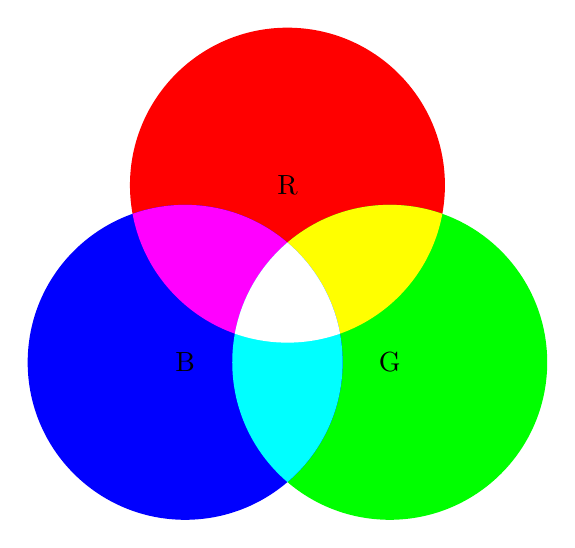
\begin{tikzpicture}

% Draws the three main circles Red, Green and Blue
\draw [draw=none, fill=red] (90:1.5) circle (2cm);
\draw [draw=none, fill=green] (-30:1.5) circle (2cm);
\draw [draw=none, fill=blue] (210:1.5) circle (2cm);

% Draws the 2 zone overlapping areas between the main circles
\begin{scope} % red + green = yellow
	\clip (90:1.5) circle(2cm);
	\draw [draw=none, fill=yellow] (-30:1.5) circle (2cm);
\end{scope} % blue + red = magenta
\begin{scope}
	\clip (210:1.5) circle(2cm);
	\draw [draw=none, fill=magenta] (90:1.5) circle (2cm);
\end{scope}
\begin{scope} % green + blue = cyan
	\clip (-30:1.5) circle(2cm);
	\draw [draw=none, fill=cyan] (210:1.5) circle (2cm);
\end{scope}

% Draws the 3 zone overlapping area in the middle
\begin{scope} % red + green + blue = white
	\clip (90:1.5) circle(2cm);
	\clip (210:1.5) circle(2cm);
	\draw [draw=none, fill=white] (-30:1.5) circle (2cm);	
\end{scope}

% Writes out the text first letter of each colour in the RGB scale in the centre of each corresponding circle
\node[draw=none] at (90:1.5) {R};
\node[draw=none] at (-30:1.5) {G};
\node[draw=none] at (210:1.5) {B};

\end{tikzpicture}
\end{document}